% Created 2011-04-26 Tue 00:56

\documentclass[english,10pt,presentation]{beamer}
\usepackage[english]{babel}
\usepackage[utf8]{inputenc}
\usepackage[T1]{fontenc}
\mode<article>
{
  \usepackage{times}
  \usepackage{mathptmx}
  \usepackage[left=1.5cm,right=6cm,top=1.5cm,bottom=3cm]{geometry}
}
\usepackage{fancybox}
\usepackage{multimedia}
\usepackage{colortbl}
\usepackage{yfonts}
\usepackage{colortbl}
\usepackage{translator}
\usepackage{times}
\usepackage{fixltx2e}
\usepackage{graphicx}
\usepackage{longtable}
\usepackage{float}
\usepackage{wrapfig}
\usepackage{soul}
\usepackage{textcomp}
\usepackage{marvosym}
\usepackage{wasysym}
\usepackage{latexsym}
\usepackage{amssymb}
\usepackage{amsmath}
\usepackage{amsfonts}
\usepackage{ifthen}
\usepackage{mypgf}
\usepackage{hyperref}

\usepackage{fixltx2e}
\usepackage{graphicx}
\usepackage{longtable}
\usepackage{float}
\usepackage{wrapfig}
\usepackage{soul}
\usepackage{textcomp}
\usepackage{marvosym}
\usepackage{wasysym}
\usepackage{latexsym}
\usepackage{amssymb}
\usepackage{amsmath}
\usepackage{amsfonts}
\usepackage{ifthen}
\usepackage{hyperref}
\usepackage{mypgf}
\providecommand{\alert}[1]{\textbf{#1}}

\title{Contracting Curve Density Algorithm}
\author{Dejan Pangercic}
\date{\today}

\usetheme{amsterdam}\usecolortheme{rose}
\begin{document}

\maketitle

\begin{frame}
\frametitle{Outline}
\setcounter{tocdepth}{2}
\tableofcontents
\end{frame}

\section{Overview}
\label{sec-1}
\begin{frame}
\frametitle{Contracting Curve Density (CCD) Algorithm}
\label{sec-1_1}
\begin{itemize}

\item a model-based image segmentation method\\
\label{sec-1_1_1}%
\item fits a parametric curve model (prior knowledge) to an image\\
\label{sec-1_1_2}%
\begin{figure}[htb]
\centering
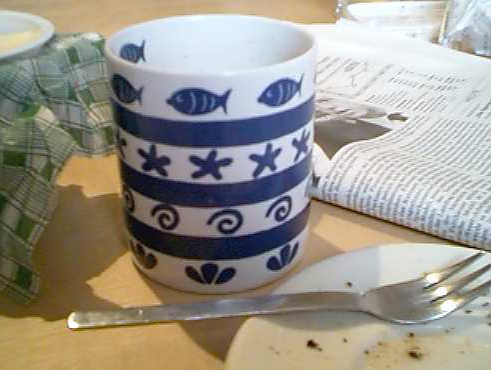
\includegraphics[width=8cm,angle=0]{/scratch/personal/doc/master_thesis/ppt/images/cup.png}
\caption{\label{fig:1}A curve fitting problem}
\end{figure}

\end{itemize} % ends low level
\end{frame}
\section{Description}
\label{sec-2}
\begin{frame}
\frametitle{Bayesian theorem}
\label{sec-2_1}

    given the prior distribution of model parameters $p(\phi)$, and
    likelihood of the model parameters given the image data
    $p(I^*|\phi)$ (here $I^{*}$ is the image data), the goal is
    maximum a posteriori estimation (MAP)
\begin{displaymath}
\mathcal{X}^2(\phi) = \mathrm{argmin}_{\phi} p(\phi|I^*)
\end{displaymath}

where 
\begin{displaymath}
p(\phi|I^*) = \frac{p(I^*|\phi) p(\phi)}{p(I^{*})}
\end{displaymath}
\end{frame}
\begin{frame}
\frametitle{Fuzzy assignment}
\label{sec-2_2}

use a probabilistic way to compute the weight $\omega$ of pixels assigned to
respective side (A and B)
\begin{figure}[htb]
\centering
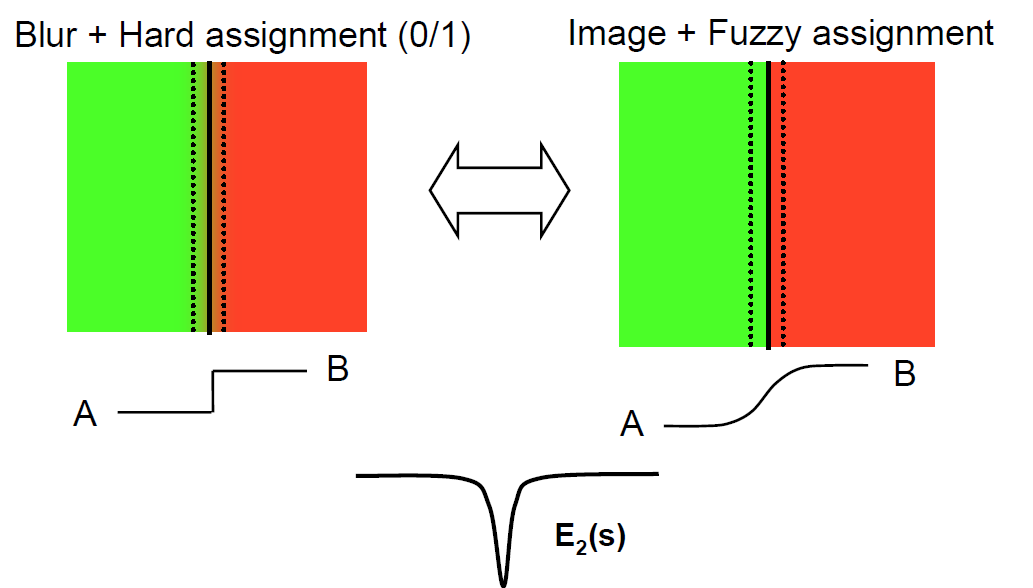
\includegraphics[width=8cm,angle=0]{/scratch/personal/doc/master_thesis/ppt/images/fuzzy.png}
\caption{\label{fig:2}Fuzzy assignment}
\end{figure}
\end{frame}
\section{Steps of CCD algorithms}
\label{sec-3}
\begin{frame}
\frametitle{Steps of CCD algorithms}
\label{sec-3_1}
\begin{alertblock}{repeat these two steps until convergence}
\label{sec-3_1_1}
\begin{itemize}

\item Learn local statistics\\
\label{sec-3_1_1_1}%
compute the pixel values and its statistics information ($I_v(\omega), m_{v}(\omega), \Sigma_v(\omega)$) from the vicinity of the expected curve based on
the current mean vector $m_{\phi}$ and the current covariance matrix $\Sigma_{\phi}$

\item Refine the estimate of the model parameter vector\\
\label{sec-3_1_1_2}%
a) Update the mean vector $m_{\phi}$ using a maximum a posteriori (MAP) criterion derived
from the local statistics
b) Update the covariance matrix $\Sigma_{\phi}$ based on the Hessian of the objective function used
in a) 



\end{itemize} % ends low level
\end{alertblock}
\end{frame}
\section{Advantages and application}
\label{sec-4}
\begin{frame}
\frametitle{Advantages and disadvantages}
\label{sec-4_1}
\begin{block}{advantages}
\label{sec-4_1_1}
\begin{itemize}

\item robust to clutter, occlusions etc\\
\label{sec-4_1_1_1}%
\item sub-pixel scale optimization\\
\label{sec-4_1_1_2}%
\item fast\\
\label{sec-4_1_1_3}%
\end{itemize} % ends low level
\end{block}
\begin{alertblock}{disadvantages}
\label{sec-4_1_2}
\begin{itemize}

\item need to initialize the hypothesis manually\\
\label{sec-4_1_2_1}%
\item not work for objects with holes\\
\label{sec-4_1_2_2}%
\end{itemize} % ends low level
\end{alertblock}
\end{frame}
\begin{frame}
\frametitle{Application}
\label{sec-4_2}
\begin{itemize}

\item Segmentation\\
\label{sec-4_2_1}%
\item Tracking\\
\label{sec-4_2_2}%
\end{itemize} % ends low level
\end{frame}

\end{document}
